
\begin{figure}
    \centering
    \begin{fullwidth}
    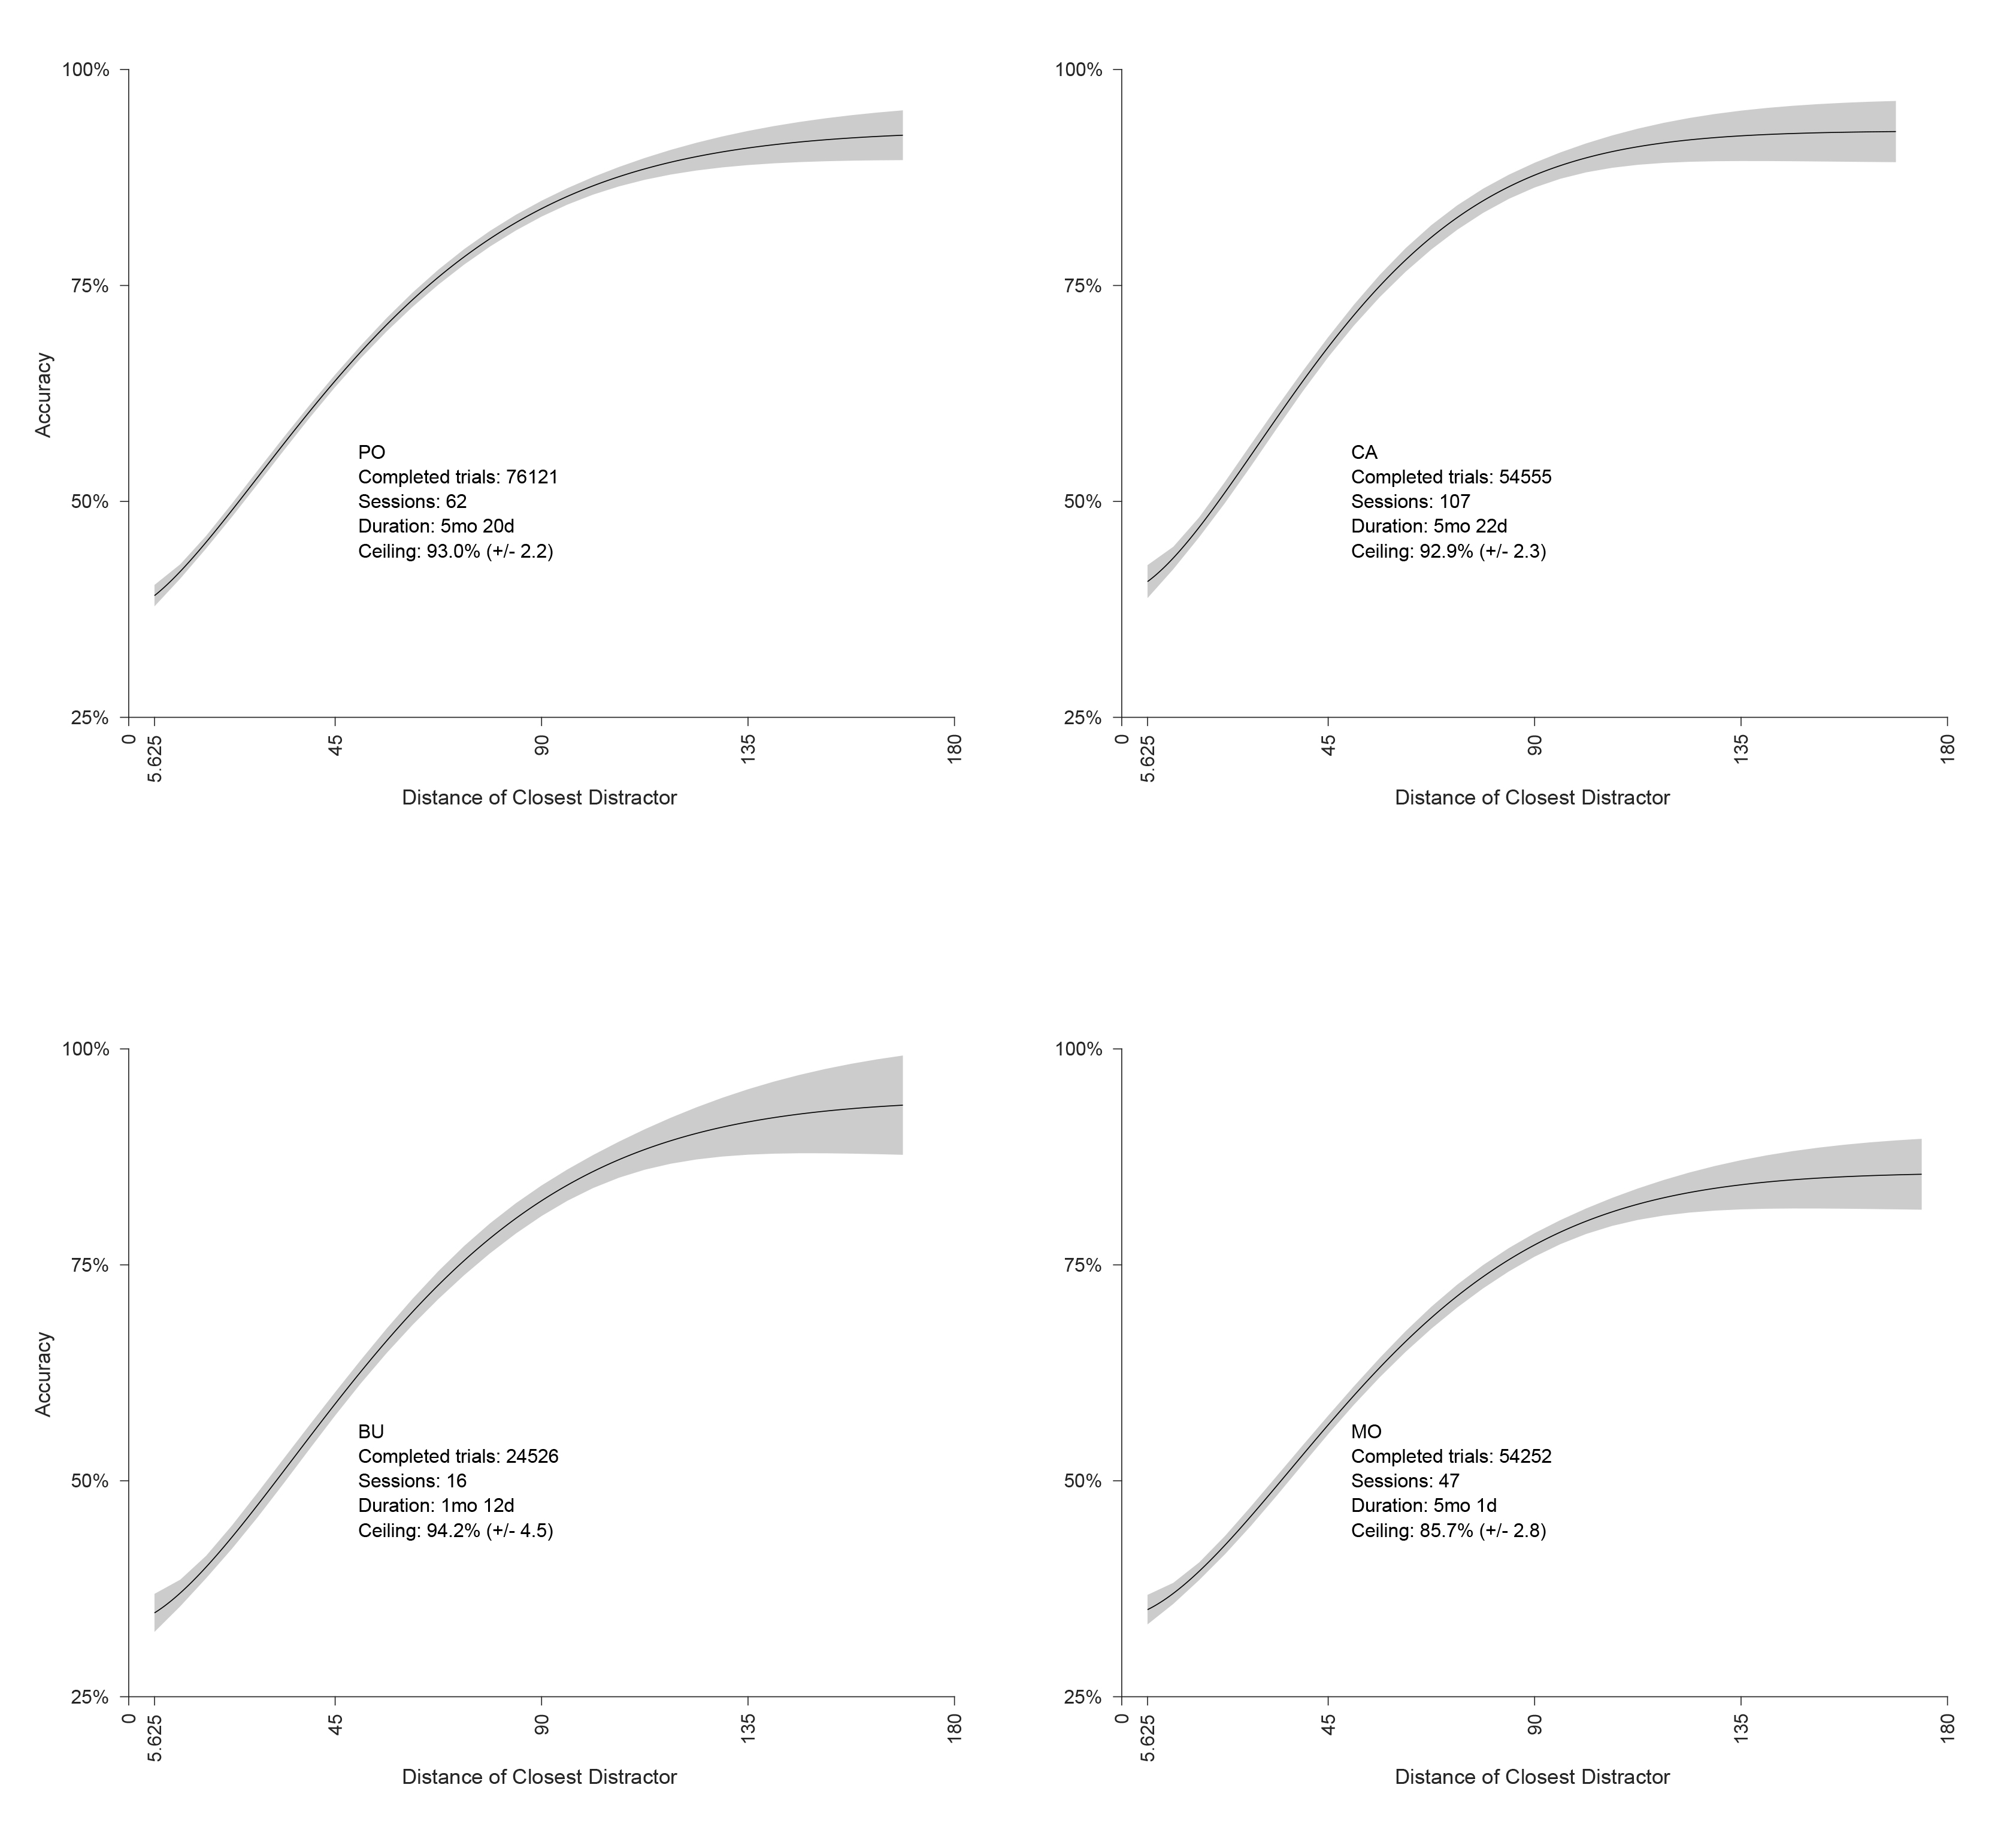
\includegraphics[width=\textwidth+4cm]{../Figures/flat/SI1_psychometric.jpg}
    \caption{\textbf{Psychometric functions for the four individual animals (PO, CA, BU, MO) on the color-matching task illustrated in Figure 1.}
    Completed trials for the four animals were: 76121; 54555; 24526; 54252.
    } 
    \label{fig:IndiDiff}
    \end{fullwidth}
\end{figure}

\begin{figure}
    \centering
    \begin{fullwidth}
    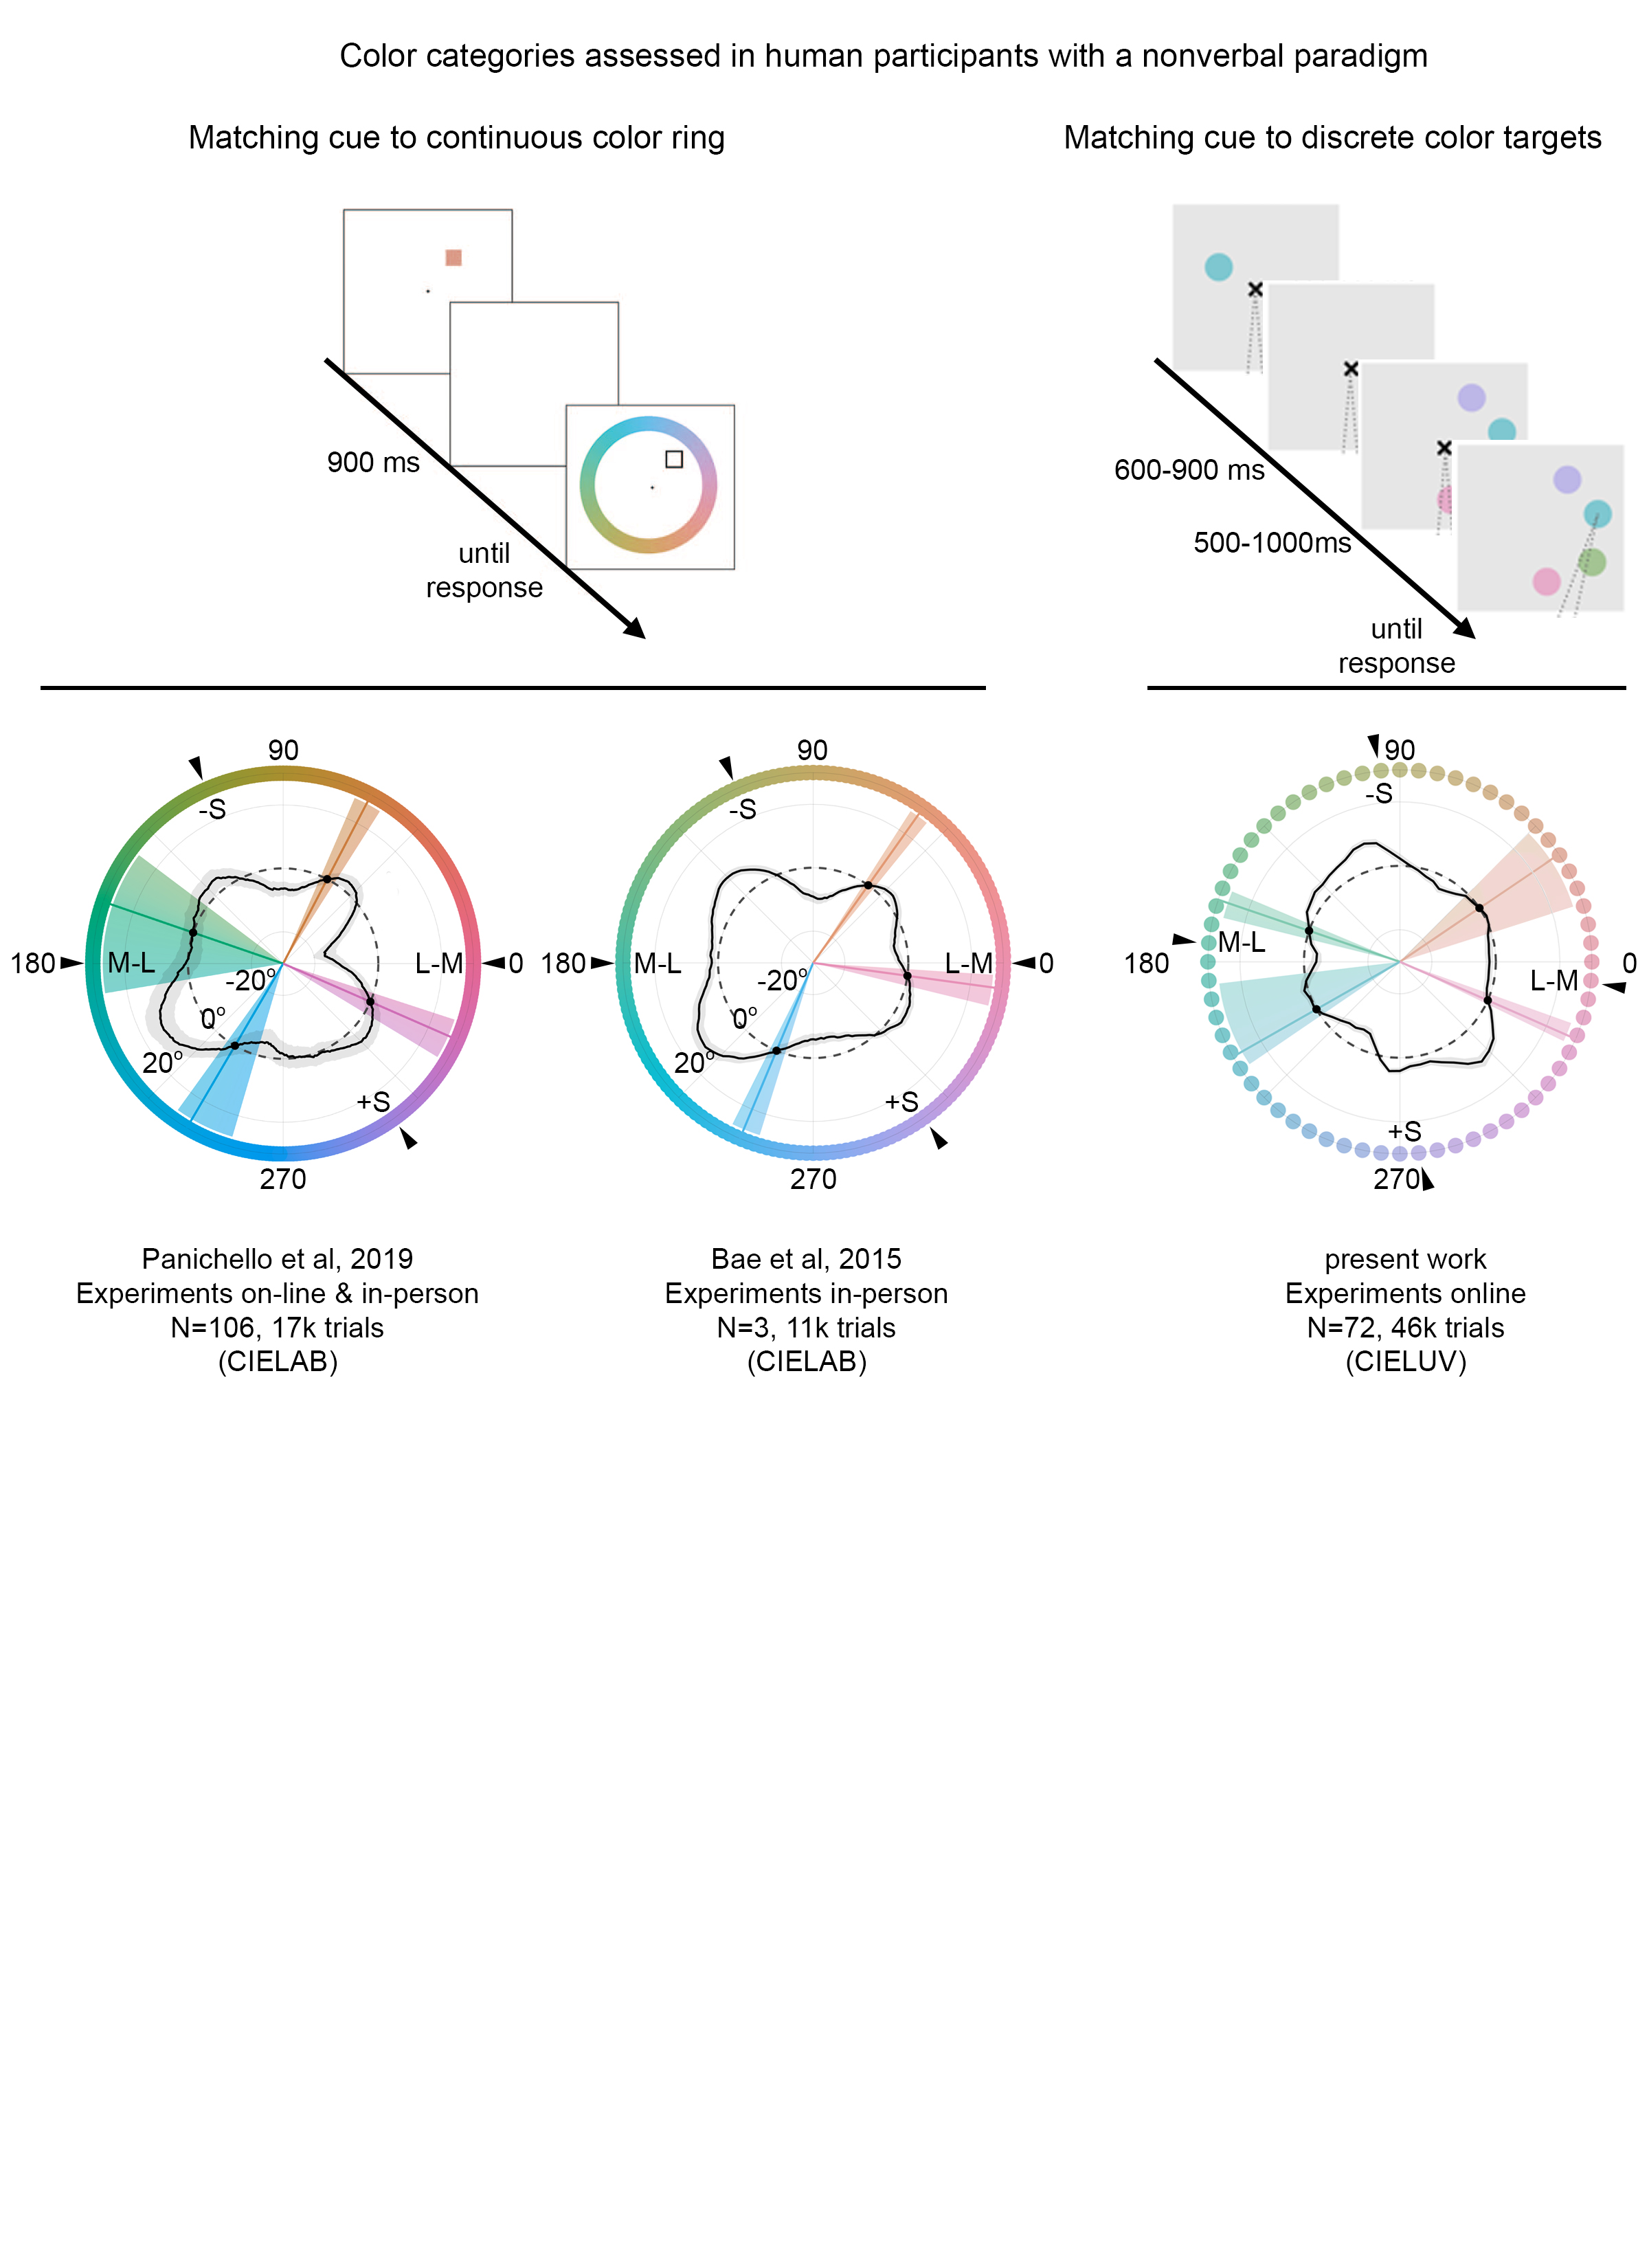
\includegraphics[width=\textwidth+4cm,trim={0 11cm 0 0},clip]{../Figures/flat/SI_Human_2.jpg}
    \caption{\textbf{Color categories assessed in human participants with a nonverbal paradigm. }
    Prior work by \citet{bae_why_2015} and \citet{panichello_error-correcting_2019} has used a task in which participants match the color of a cue to a continuous ring of colors; those published results were obtained with a combination of in-person experiments and on-line experiment, with a memory delay and without. The results are broadly consistent, recovering four color categories by mixture-model analysis, corresponding to blue, green, orange and pink. 
    Note that the data from \citep{bae_why_2015} shown in the figure were from just three participants, engaged in a task that had a memory delay; those authors confirmed the results in more subjects with a version of the task that omitted the memory delay period (the cue and the match-option color wheel were presented simultaneously). The present work adapted the paradigm so that the match options in each trial were four discrete targets randomly drawn from 64 colors sampling the color space. The data shown in this figure were obtained in human participants, with experiments conducted online with Amazon Mechanical Turk. These results are again broadly consistent with the prior work using the continous-matching ring in recovering, by mixture analysis, four significant categories corresponding to blue, green, orange, and pink. We note that the discrete-matching task recovers a trend for a fifth category that would correspond to “purple”; close inspection of the results in \citep{bae_why_2015, panichello_error-correcting_2019} and in studies of human infants \citep{skelton_biological_2017} also show evidence of this trend. The stimuli in the \citep{bae_why_2015, panichello_error-correcting_2019} were defined in CIELAB, while the stimuli in the present work were defined in CIELUV; this difference in color space is associated with a slight clockwise rotation of the cone-opponent axes. The S axis poles provide a useful landmark; they are associated with negative slopes in all three data sets.
    } 
    \label{fig:Human}
    \end{fullwidth}
\end{figure}

\begin{figure}
    \centering
    \begin{fullwidth}
    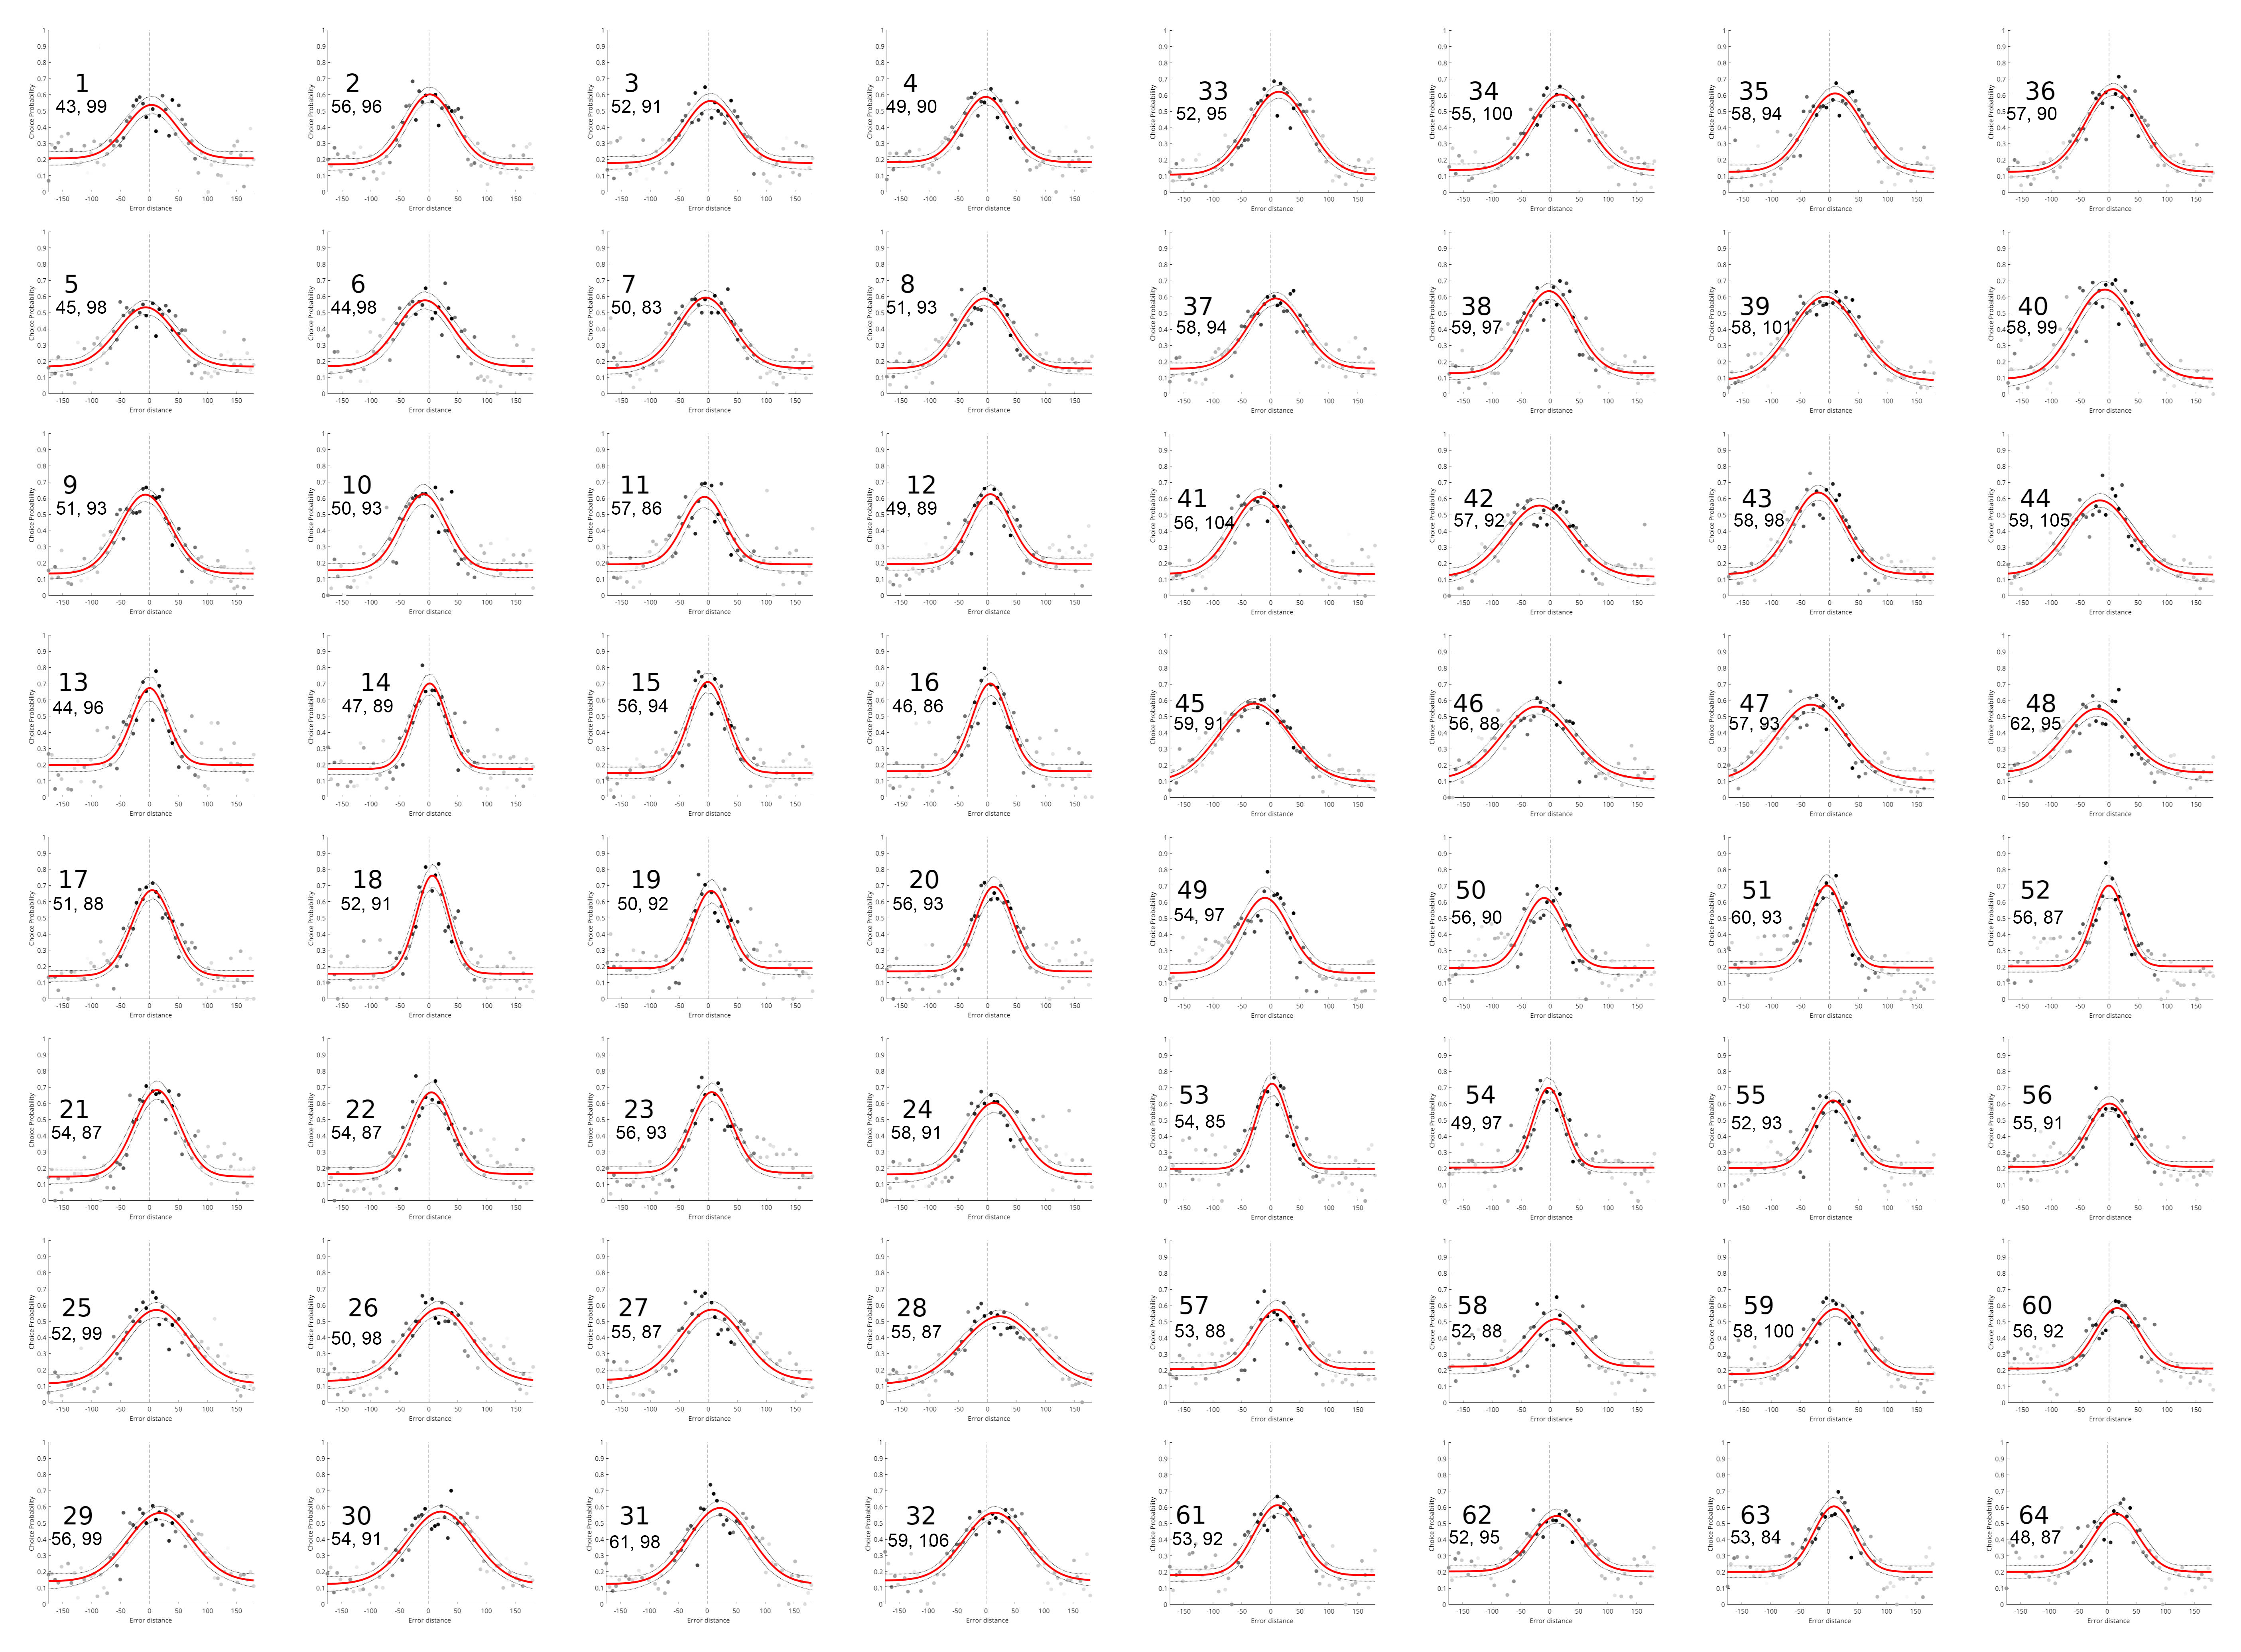
\includegraphics[width=\textwidth+4cm]{../Figures/flat/SI3_MMBreakOut_2.jpg}
    \caption{\textbf{Gaussian fits from the Mixture Model.}
    Each trace shows the Gaussian fit for one of the 64 target colors (large number in each panel corresponds to the cue color) used in the color-matching task, as per Equation 1; data averaged over four animals. The extent to which each data point is black versus white indicates the number of trials that provided that choice option, normalized for each cue (the pair of smaller numbers below the cue-color number provides the range: the larger number corresponds to the black symbol, and the smaller number to white); see Methods for how the curves were fit to the data. 
    } 
    \label{fig:MMBreakOut}
    \end{fullwidth}
\end{figure}

\begin{figure}
    \centering
    \begin{fullwidth}
    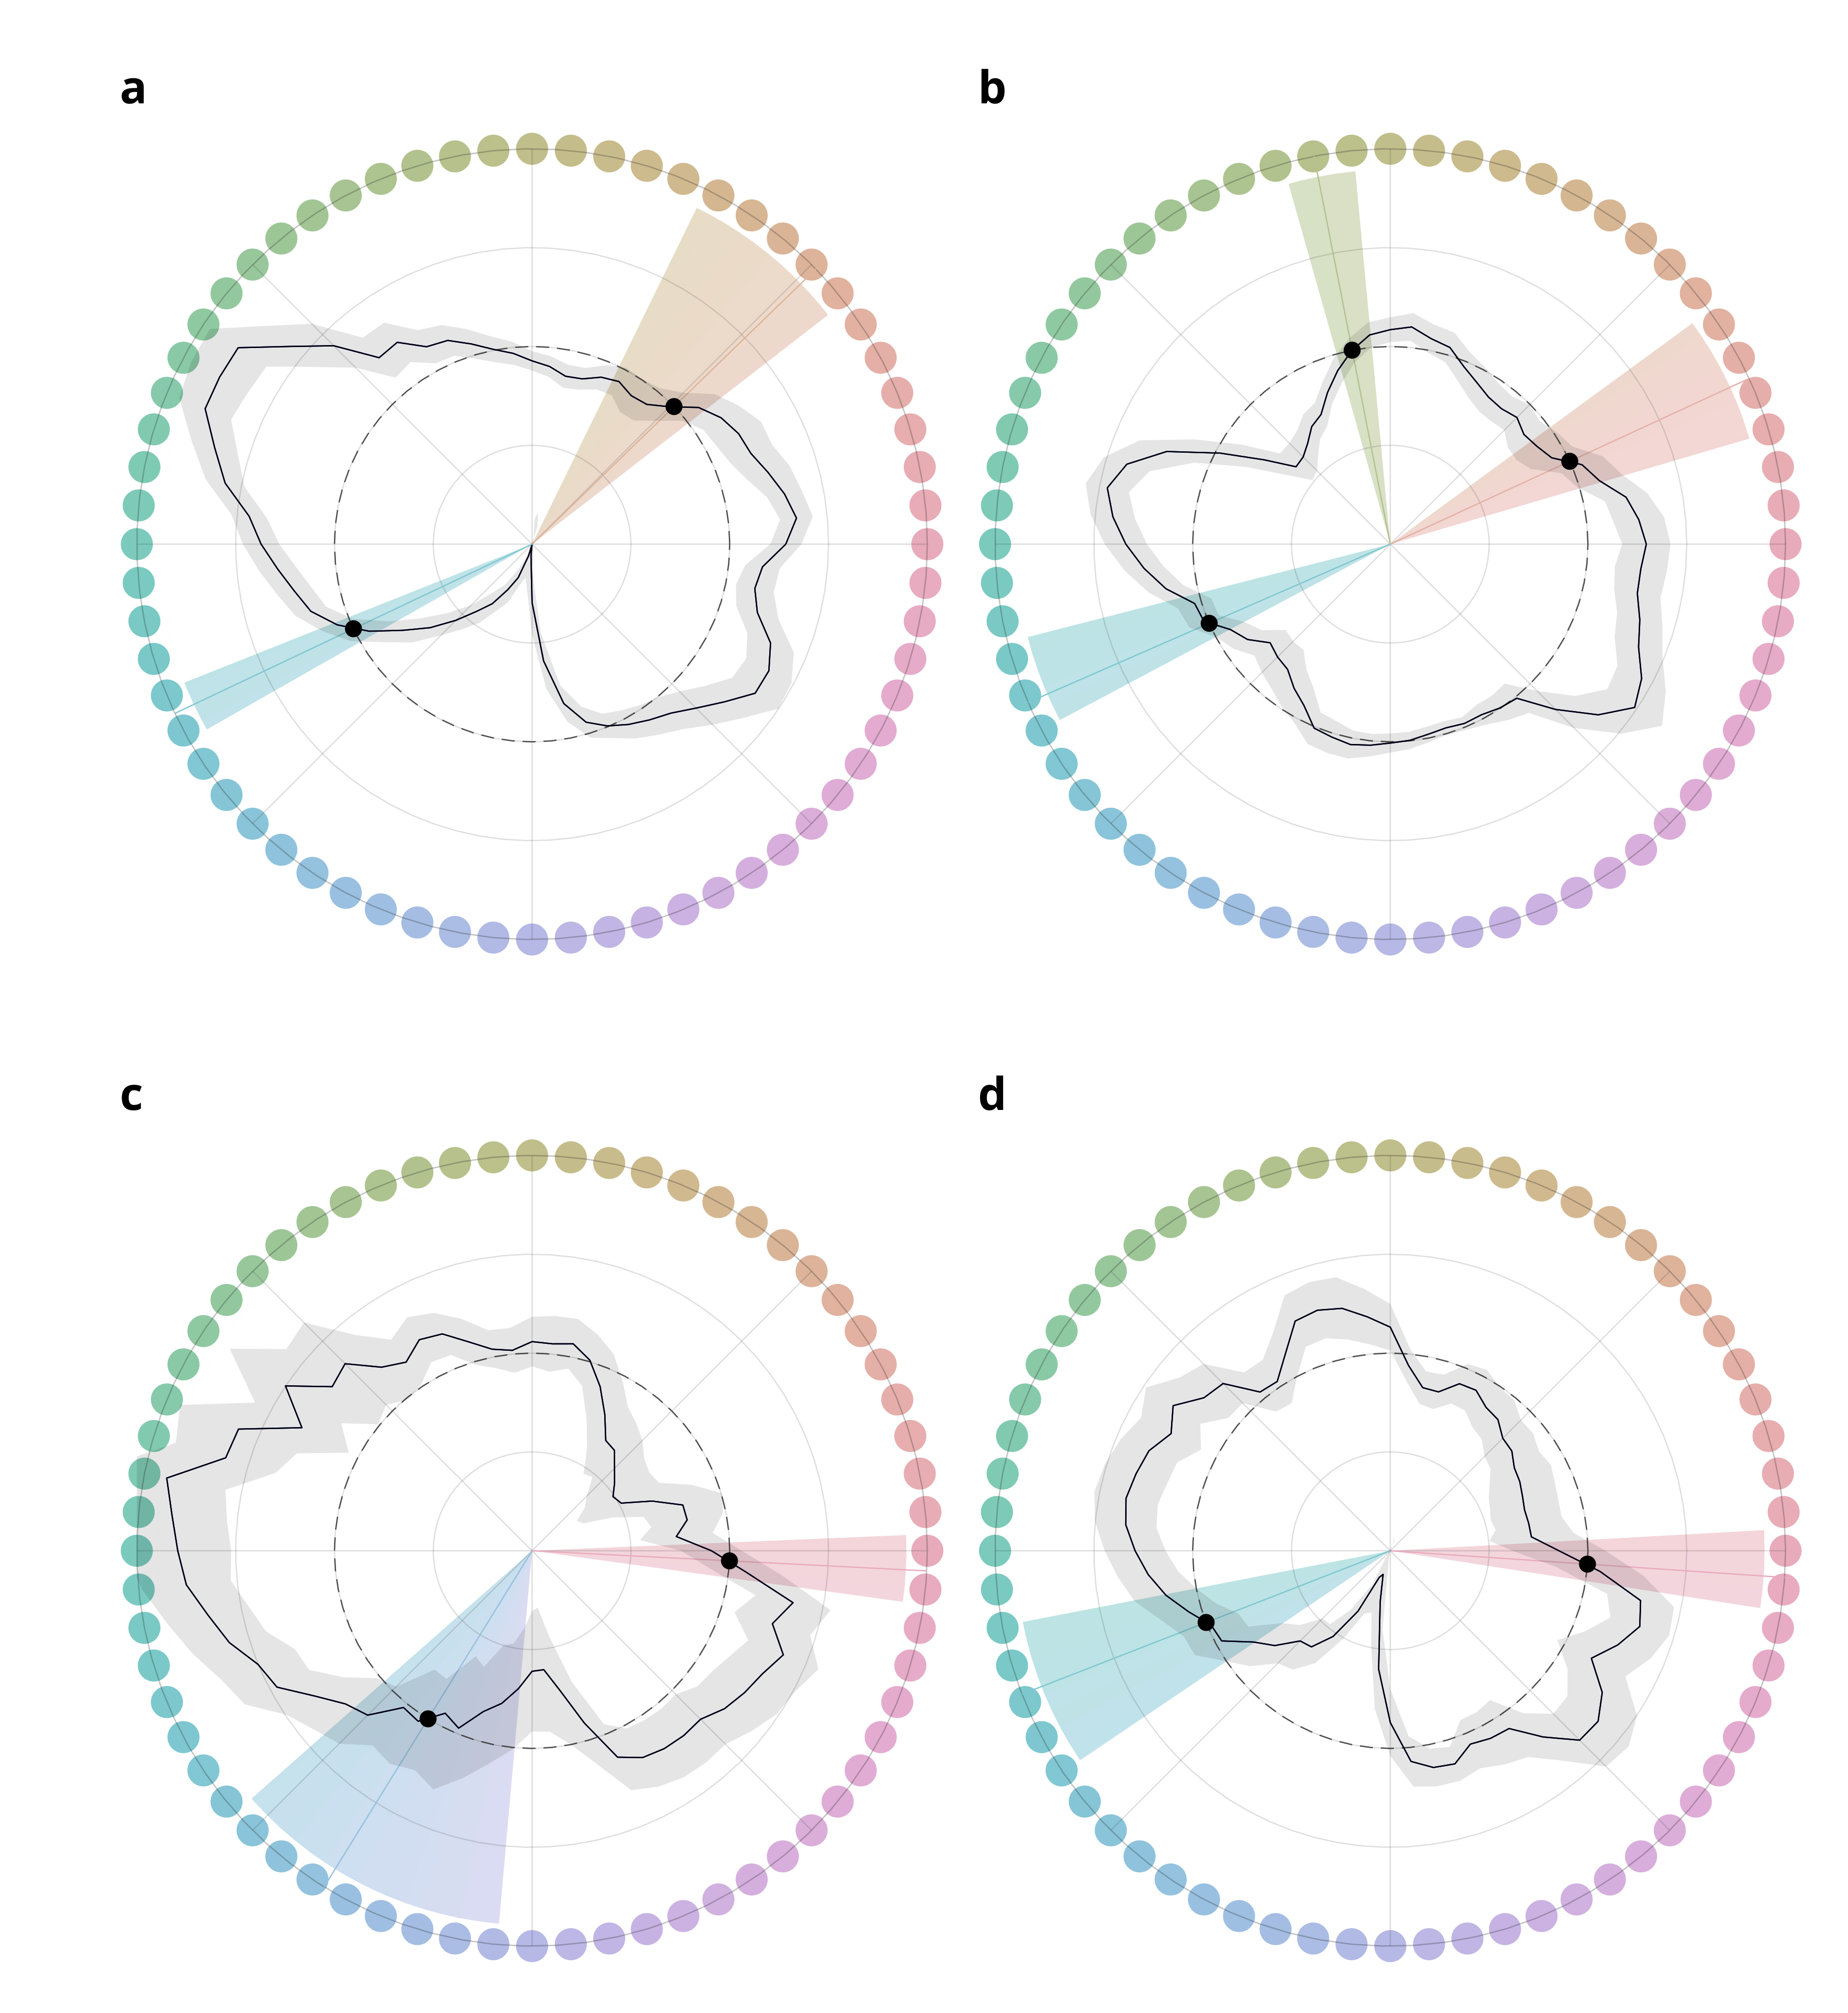
\includegraphics[width=\textwidth+4cm]{../Figures/flat/SI4_MM.jpg}
    \caption{\textbf{Mixture-model analysis of the individual data for the four animals in the color-matching task.}
    Data shown in the same format as Figure 2c.
    All data for each animal is included (in contrast to Figures 2bc where data were subsampled to ensure equal contributions from each animal).
    } 
    \label{fig:IndiMM}
    \end{fullwidth}
\end{figure}

\begin{figure}
    \centering
    \begin{fullwidth}
    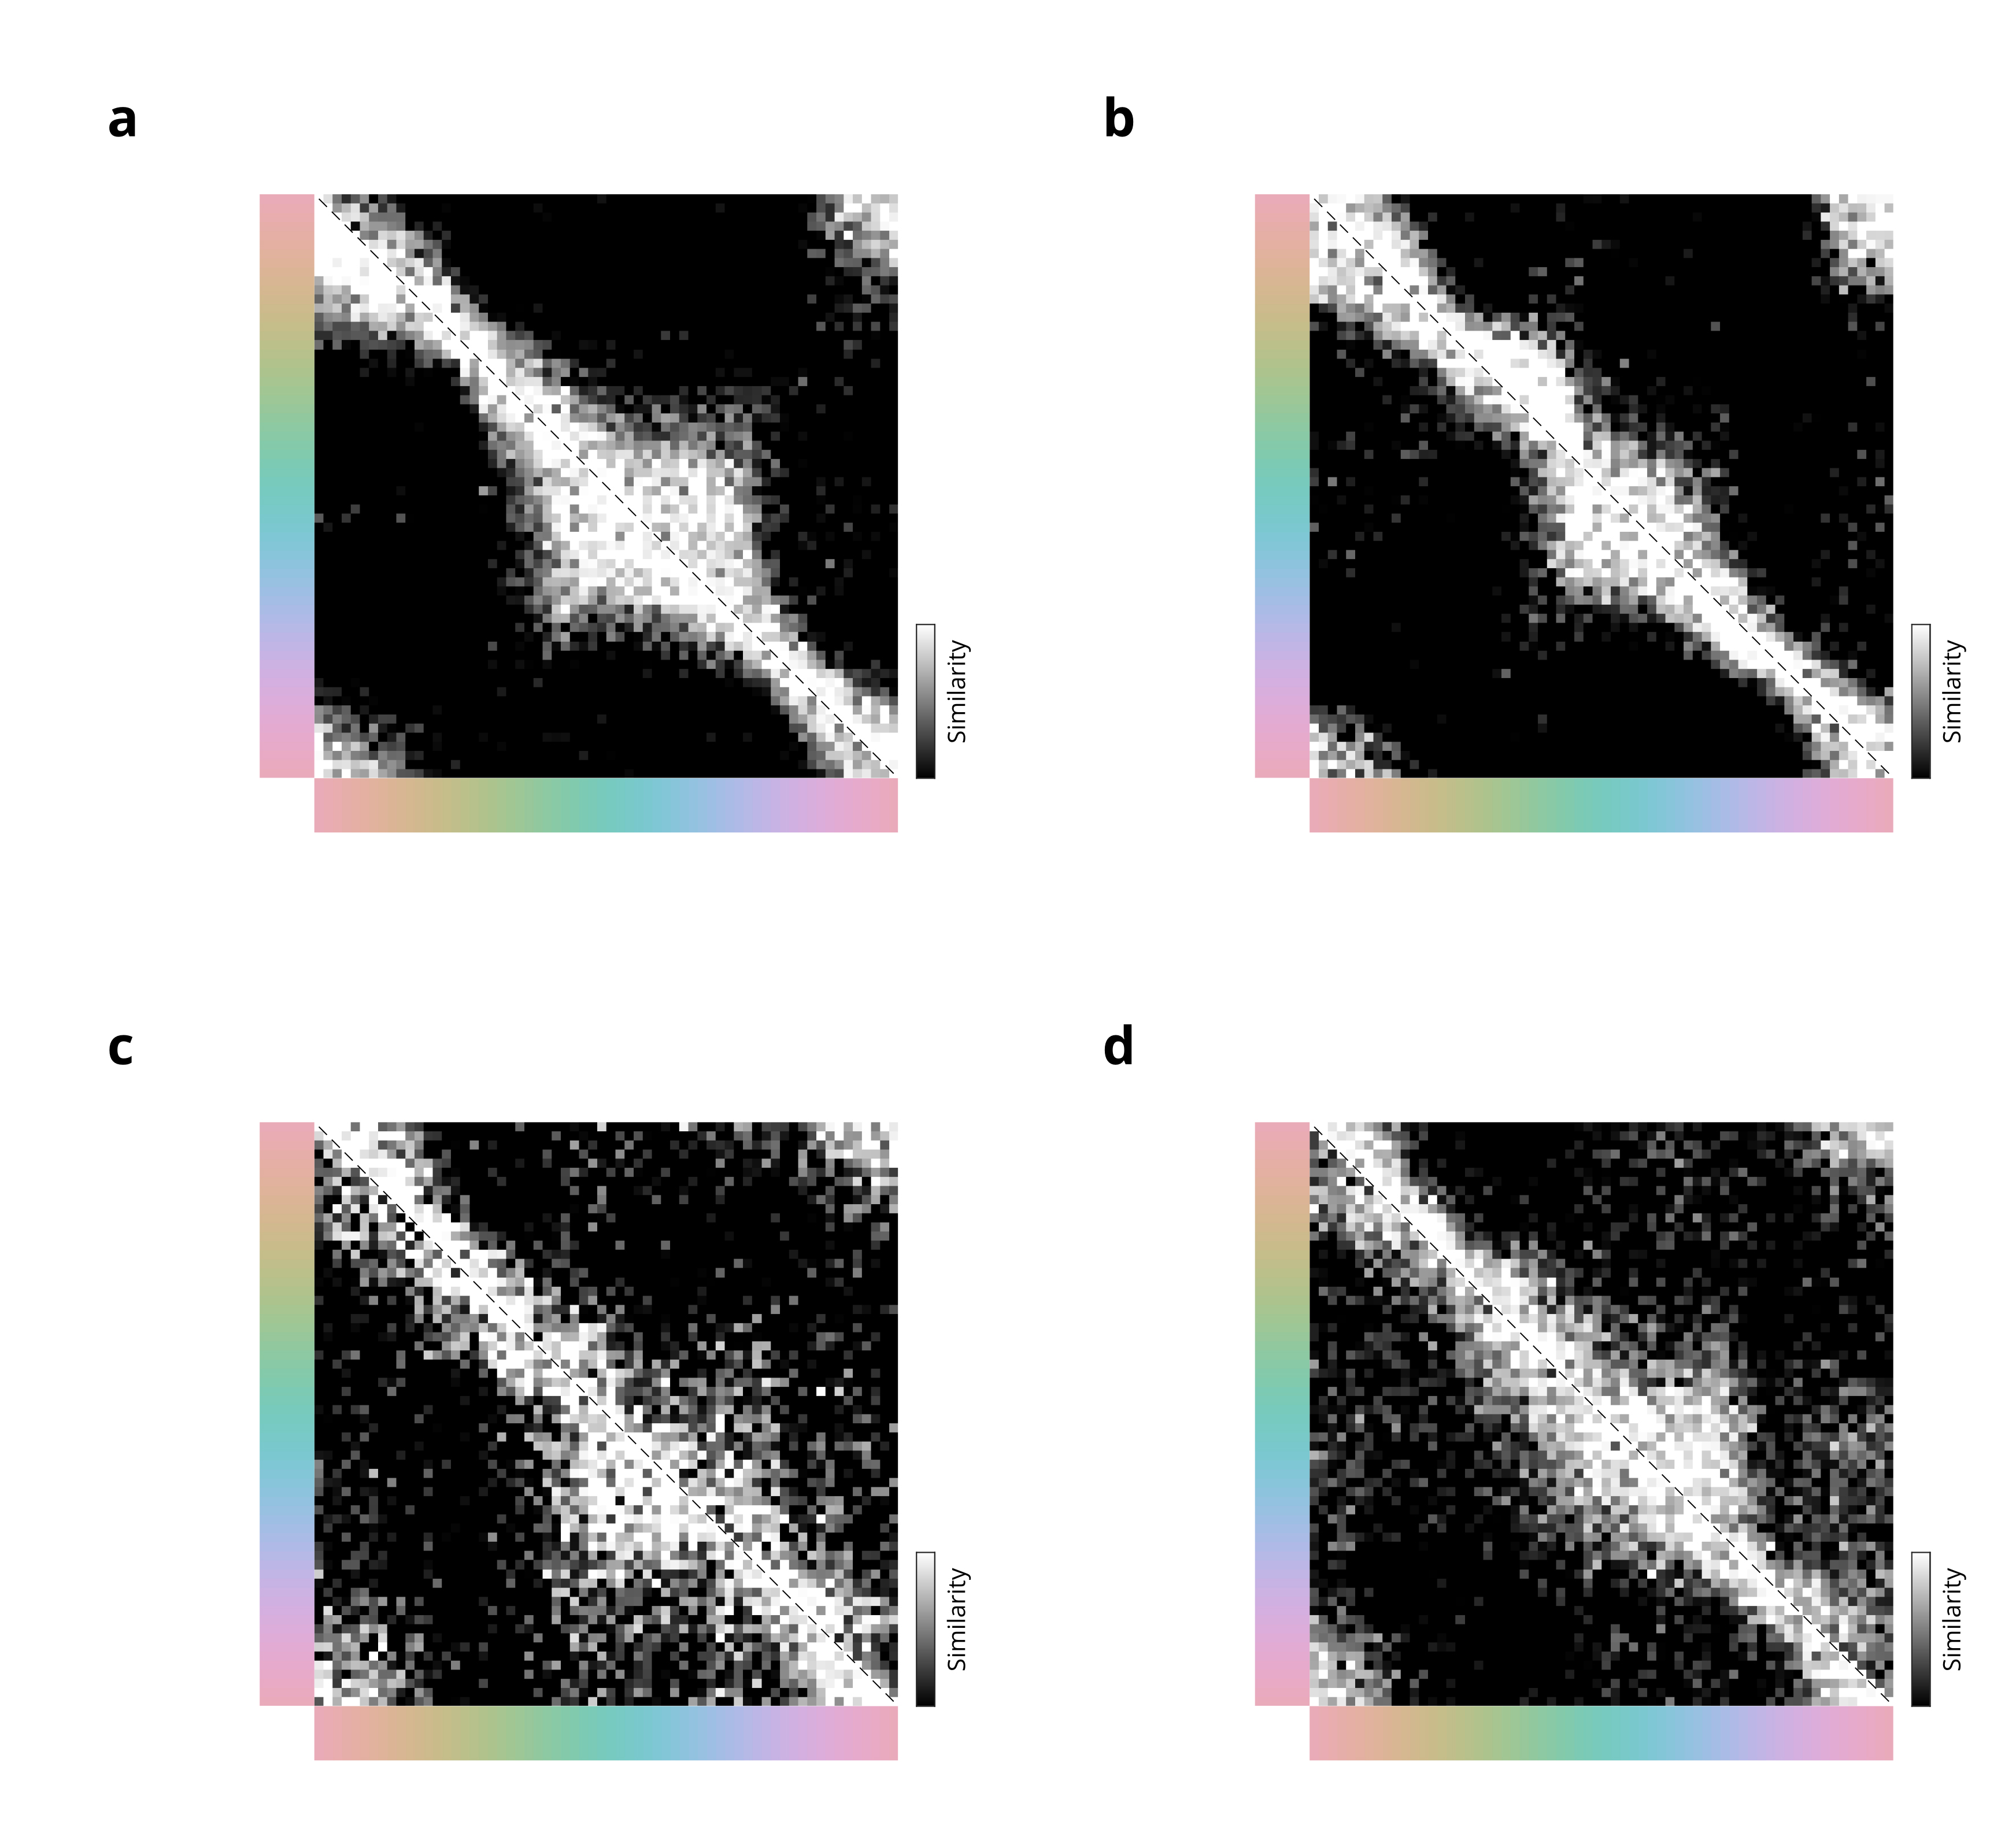
\includegraphics[width=\textwidth+4cm]{../Figures/flat/SI5_IndTCCv.jpg}
    \caption{\textbf{Similarity matrices for free similarity matrix models, fit to individual data.}
    The order of the plots is the same as the order in other figures, PO, CA, BU, MO. 
    These plots use the full set of data for each animal.
    See Figure 3ab for data averaged across animals, with data subsampled to ensure the same amount of data per animal.
    } 
    \label{fig:IndiTCC}
    \end{fullwidth}
\end{figure}

\begin{figure}
    \centering
    \begin{fullwidth}
    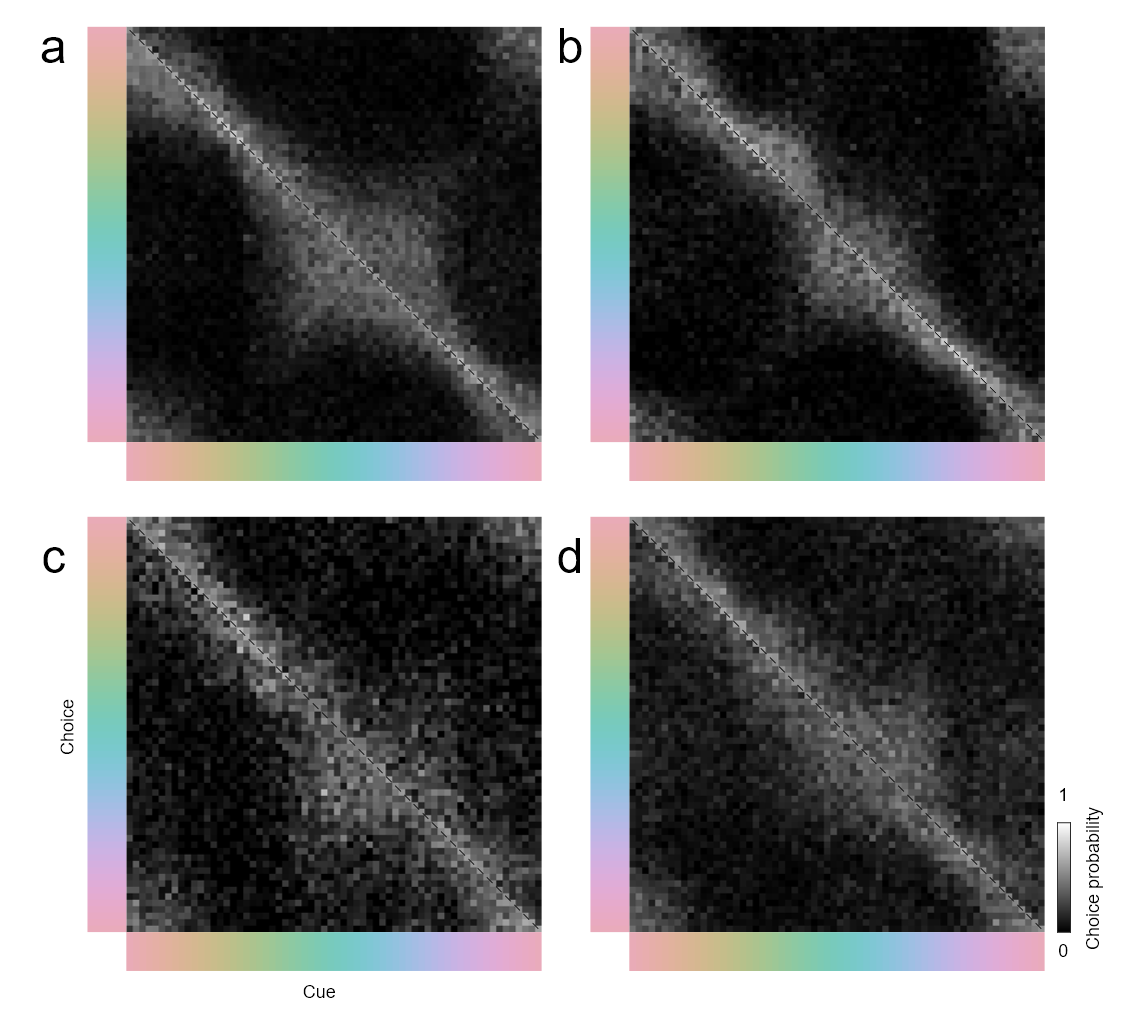
\includegraphics[width=\textwidth+4cm]{../Figures/flat/SI6_choiceMatrices.png}
    \caption{\textbf{Choice probability matrices for free similarity matrix models, for the four individuals.}
    As per the similarity matrices presented, each column represents a cue, and each row represents a choice. 
    Here, however, rather than the similarity between cue/choice pairs we show the probability of selection. 
    Whereas the similarity matrix is the output of model fitting, this matrix is derived more directly from the data: each cell is simply the number of times a particular choice was made divided by the number of times that choice was an option. 
    The identity line, representing correct options, appears artifically inflated (see Methods for further information).
    } 
    \label{fig:choiceProbabilityMatrices}
    \end{fullwidth}
\end{figure}

